\chapter{Growing a Social Page as a Distribution System}

This chapter follows a School of Hard Knocks entrepreneurship lesson, curated by LazyingArt LLC through Video2Book, on growing Instagram and Facebook pages. The lecture is not a theory of social media in the abstract. It is an operator's account: a practitioner says that after years of running pages, a repeatable pattern became visible. We will keep that practical rhythm. First comes consistency, then content supply, then short-form distribution, then audience routing, then the platform frictions and calls to action that turn attention into growth.

\section{The Claim: Growth Becomes Repeatable}

The speaker begins with a claim of practice-based authority. He has been in digital marketing for about four years, has worked on many social pages and channels, and has generally been able to grow them. But he distinguishes general experience from a more recent recognition: in the previous six months or so, he began to see a few ingredients that behaved like a formula for fast growth.

We should be careful with the word ``formula.'' It is not a guarantee. It is an operating model. A page grows when a set of conditions are kept active together:
\begin{equation}
\text{growth system}
=
\text{cadence}
+
\text{content supply}
+
\text{distribution format}
+
\text{audience signal}
+
\text{feedback}.
\end{equation}

That is also the order of the lecture. We first ask how often the page must act. Then we ask where enough content comes from. Then we ask which formats travel beyond the existing audience. Finally we ask how the platform is signaled, where friction enters, and how the creator keeps testing.

\section{Consistency as Momentum Preservation}

The first tip is consistency, and the speaker calls it the most important because every later tactic rests on it. Once a page has momentum, the job is to keep that momentum alive. Posting is not merely publication; it is repeated contact with the audience and repeated evidence to the platform that the page is active.

The practical cadence is stated directly:
\begin{equation}
\text{posting cadence} \in
\{\text{daily},\ \text{every other day}\}.
\end{equation}

The motivation is top-of-mind awareness. Loyal followers remain engaged because the page keeps appearing. In a simple reconstructed model, we can write momentum as a quantity that decays unless renewed:
\begin{equation}
M_{n+1}
=
\alpha M_n + E_n,
\qquad 0 < \alpha < 1.
\end{equation}
Here $M_n$ is page momentum after cycle $n$, and $E_n$ is the engagement created by the next post. This equation is not spoken in the lecture; it is a compact way to preserve the speaker's mechanism. If $E_n$ disappears for too long, the old momentum decays. If posting continues, each new response helps replenish the system.

This is why the next problem appears immediately. A daily or every-other-day cadence is easy to recommend and hard to sustain. We need a content pipeline.

\section{Solving the Content Supply Problem}

The speaker's first answer is to look outward. Use competitors and similar pages to understand what is already working. Look at relevant hashtags, top posts, and trending material. This is not a call to copy blindly; it is an instruction to observe the market.

\subsection{Question \& Answer}

\paragraph{Question.}
How do we find enough content without simply stealing from other pages?

\paragraph{Answer.}
The lecture pauses to set an ethical boundary. Similar pages can be a source of ideas, and in some cases a source of concrete material, but credit matters. The speaker gives the example of reposting an Elon Musk quote: if he shares it with his own audience, he credits the original page in the description. The page using the post gets content; the source page gets exposure. The point is not theft disguised as strategy, but credited borrowing and adaptation.

The same logic applies to search. If we search an industry plus ``content ideas,'' look through image results, and scan articles listing dozens of post concepts, we are building a library of prompts. The output still has to be fitted to the page.

The speaker then gives a useful classification of content demand:
\begin{equation}
\text{content demand}
=
\{\text{education},\ \text{entertainment}\}.
\end{equation}
People usually look at pages either to learn something or to be entertained. That simple split turns ideation into a feedback process. We post, inspect the analytics, and then model what worked.

\begin{align}
\text{publish} &\longrightarrow \text{measure response},\\
\text{measure response} &\longrightarrow \text{separate working patterns},\\
\text{working patterns} &\longrightarrow \text{model and replicate}.
\end{align}

This is the first real feedback loop in the lecture. Consistency supplies enough trials; analytics decides which trials deserve repetition.

\section{Reels as Organic Distribution}

The second tip is to use reels. The speaker presents reels as the best current route to large organic reach on Instagram and Facebook. The important point is that this reach is not limited to the size of the existing audience. In his framing, a page with five followers and a page with five hundred thousand followers both have access to a format that the platforms may distribute broadly.

The lecture's practical inequality is:
\begin{equation}
\text{potential reach of reels}
>
\text{potential reach of static posts}.
\end{equation}
This is not a universal mathematical law. It is a platform observation: short-form video has more surface area for recommendation.

The next transition is to TikTok. The transcript is briefly garbled here, but the intended move is clear. TikTok is treated as a laboratory for short-form content because creators there have refined the format. If we are already making Instagram and Facebook reels, the same short-form thinking can also be used on TikTok.

A concrete threshold appears:
\begin{equation}
F_{\text{TikTok monetization}}
=
10{,}000\ \text{followers}.
\end{equation}
The threshold is not the heart of the argument. It simply adds another reason to think about short-form video as an asset that can travel across platforms.

The speaker then adds a caveat about local businesses versus theme pages. For a theme page such as rap or business, reposting or adapting viral material may be part of the workflow, provided the original creator is tagged. Again the lecture returns to the same constraint: leverage existing attention, but do not erase the source.

\section{Hashtags as Audience Routing}

The third tip is that hashtags matter, especially while a page is still getting off the ground. The speaker gives two practical counts:
\begin{align}
H_{\text{static post}} &\approx 8\text{--}10,\\
H_{\text{video/reel}} &\approx 6.
\end{align}

The important condition is relevance. A hashtag is not decoration. It is a topic signal. The speaker's example is an investing hashtag. If a post tagged with investing begins to get engagement, the platform can infer that people who usually respond to investing content are responding to this post too. That produces an audience-routing mechanism.

\subsection{Question \& Answer}

\paragraph{Question.}
Why do relevant hashtags matter if the platform is already recommending content?

\paragraph{Answer.}
They matter because they help the platform decide where to test the post. In the lecture's explanation, the hashtag-driven signal can do two things. First, it can help move the content onto Explore for people associated with that topic. Second, it can help push the content onto the home feeds of people who do not already follow the page. The mechanism is not ``hashtag equals growth.'' The mechanism is relevant signal, early engagement, wider routing.

\begin{figure}
\centering

\includegraphics[width=\linewidth]{lecture_176_figure_02.png}
\caption{Reel and post insights used as visual evidence for reach beyond current followers.}
\end{figure}

The screenshot preserves the concrete analytics context. On the right Post Insights panel, the clearest visible values are:
\begin{align}
R_{\text{post}} &= 23{,}424,\\
R_{\text{followers}} &= 17{,}478,\\
R_{\text{non-followers}} &= 5{,}946.
\end{align}
The follower and non-follower counts add back to the displayed reach:
\begin{equation}
17{,}478 + 5{,}946 = 23{,}424.
\end{equation}

From these visible values we can compute the non-follower share:
\begin{align}
\frac{R_{\text{non-followers}}}{R_{\text{post}}}
&=
\frac{5{,}946}{23{,}424} \\
&\approx 0.254.
\end{align}
Thus, in the visible example, roughly one quarter of the reached accounts were not already followers. This percentage is a reconstruction from the screenshot, not a number spoken by the lecturer.

The mechanism can be redrawn as a narrow flow suitable for a pocket layout:
\begin{figure}
\centering
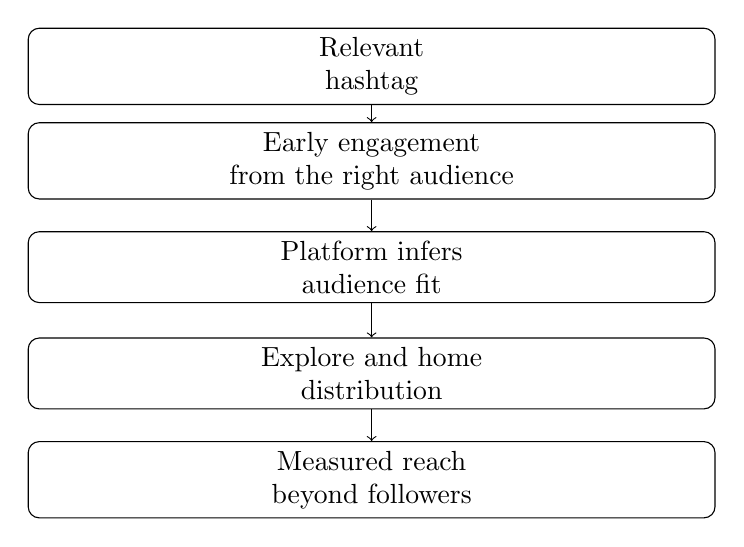
\begin{tikzpicture}
\node[draw, rounded corners, align=center, text width=0.70\linewidth] (a) at (0,0) {Relevant\\hashtag};
\node[draw, rounded corners, align=center, text width=0.70\linewidth] (b) at (0,-1.20) {Early engagement\\from the right audience};
\node[draw, rounded corners, align=center, text width=0.70\linewidth] (c) at (0,-2.55) {Platform infers\\audience fit};
\node[draw, rounded corners, align=center, text width=0.70\linewidth] (d) at (0,-3.90) {Explore and home\\distribution};
\node[draw, rounded corners, align=center, text width=0.70\linewidth] (e) at (0,-5.25) {Measured reach\\beyond followers};

\draw[->] (a) -- (b);
\draw[->] (b) -- (c);
\draw[->] (c) -- (d);
\draw[->] (d) -- (e);
\end{tikzpicture}
\caption{Hashtags interpreted as audience-routing signals.}
\end{figure}

The same frame also shows approximate impressions and traffic-source values. These are useful as visual evidence, but the small text is less certain than the main reach counts:
\begin{align}
\text{impressions} &\approx 23{,}749,\\
\text{from Home} &\approx 17{,}415,\\
\text{from Explore} &\approx 5{,}283,\\
\text{from Profile} &\approx 795,\\
\text{from Other} &\approx 79.
\end{align}

A compact table captures the values we can safely use in the chapter:
\begin{table}
\centering
\begin{tabular}{ll}
\hline
Quantity & Value or rule \\
\hline
Post accounts reached & $23{,}424$ \\
Followers reached & $17{,}478$ \\
Non-followers reached & $5{,}946$ \\
Non-follower share & $\approx 25.4\%$ \\
Static-post hashtags & $8\text{--}10$ \\
Video/reel hashtags & $\approx 6$ \\
\hline
\end{tabular}
\caption{Metric summary for the hashtag and reach mechanism.}
\end{table}

The speaker adds one more caution: be patient. Hashtags may not seem powerful at the beginning, but in his account they are one of the factors that help the page get routed to the right audience. The clean mathematical summary is:
\begin{equation}
\text{relevance} + \text{engagement}
\longrightarrow
\text{better audience routing}.
\end{equation}

\section{Friction, Limits, and Calls to Action}

After the hashtag mechanism, the lecture turns to platform friction. The next warning is about TikTok watermarks. The speaker says Instagram and Facebook do not seem to like the TikTok logo and watermark on uploaded videos. His observation is that reach improved after he downloaded videos without the watermark before posting them elsewhere.

We can write the claim as a cautious inequality:
\begin{equation}
\text{reach without watermark}
>
\text{reach with TikTok watermark}.
\end{equation}
This should be read as an anecdotal platform observation, not a controlled experiment. Still, it fits the chapter's larger logic: remove anything that makes the platform less likely to distribute the content.

The next lever is specific to Facebook. If someone reacts to a video or photo, the page owner can go to the reactions and invite that person to like the page. The speaker gives a practical batch size:
\begin{equation}
I_{\text{Facebook invites}}
\approx
200\text{--}300
\quad
\text{people per batch}.
\end{equation}
He also gives the caution from experience:
\begin{equation}
T_{\text{invite restriction}}
\approx
48\ \text{hours}.
\end{equation}
That restriction followed from overusing the invite feature. The lesson is not to avoid the feature; it is to use it inside the platform's tolerance.

The final operating lever is the post description. For static posts, the speaker suggests questions: What are your thoughts? What are your opinions? What would you choose? For videos, he suggests follower prompts such as ``follow to join the team'' or ``follow to join the movement.'' The description is a small piece of text, but it can change the next action:
\begin{equation}
\text{description prompt}
\longrightarrow
\{\text{comments},\ \text{follows},\ \text{watch time}\}.
\end{equation}

This is where the lecture's practical voice matters. The advice is not merely to ask for engagement. It is to make the next action obvious: comment, follow, keep watching, or join the page's larger identity.

\section{Testing as the Final Operating Rule}

The closing move is experimentation. Try new ideas, try new tactics, and keep testing whatever might grow the page. This final beat prevents the lecture from becoming a fixed checklist. The numbered tips are a starting system, but the page still has to learn from its own audience.

The complete loop is:
\begin{enumerate}
\item Post daily or every other day.
\item Study competitors, adjacent pages, hashtags, search results, and prior winners.
\item Credit reused material and adapt ideas to the page.
\item Prefer formats, especially reels, that have stronger organic distribution.
\item Use relevant hashtags as audience-routing signals.
\item Remove platform friction, including watermarks when reposting short-form video.
\item Invite reachable Facebook reactors within practical limits.
\item Use descriptions to prompt comments, follows, and watch time.
\item Read the analytics and repeat.
\end{enumerate}

In compact form:
\begin{equation}
\text{growth}
=
\text{creative trials}
+
\text{measured feedback}
+
\text{disciplined repetition}.
\end{equation}
That is the entrepreneurial structure of the lecture. Creativity supplies variants. The platform supplies feedback. Discipline keeps the experiment running long enough for patterns to appear.

\section{Summary}

The lecture begins with a claim that social page growth has become repeatable, then builds the operating system step by step. Consistency preserves momentum. Competitor research, credited reuse, search, and analytics solve the content-supply problem. Reels create stronger organic distribution possibilities. Relevant hashtags help route content toward the right audience, and the visible analytics frame shows how reach can include a measurable non-follower component.

The final tactics are operational: avoid watermarks that may suppress distribution, invite Facebook reactors within platform limits, and use descriptions to prompt engagement and follows. The strongest lesson is not a single hack. It is a loop: create, publish, route, observe, adapt, and repeat.